\documentclass{beamer}
%\usepackage{beamerarticle}
\usepackage{heppennames}
\usepackage{hepnicenames}
\usepackage{graphicx} 
\usepackage{multirow}
\usepackage{amsbsy,amsmath,amssymb}
\usepackage{booktabs}
% ********** Styl prezentacji **********
\mode<presentation>
{
	\usetheme{Singapore}
  \setbeamercovered{transparent}
   \setbeamertemplate{footline}[frame number] 
  \setbeamertemplate{navigation symbols}{ 
  \insertslidenavigationsymbol
  \insertframenavigationsymbol
  \insertsubsectionnavigationsymbol
  \insertsectionnavigationsymbol
  \insertdocnavigationsymbol
  \insertbackfindforwardnavigationsymbol
  \hskip 0.3cm
  %\insertframenumber / \inserttotalframenumber  % <<< frame #
  %\insertpagenumber / \insertpresentationendpage % <<< page #
} 
}

\usepackage[english]{babel}
\usepackage[latin1]{inputenc}

% font definitions, try \usepackage{ae} instead of the following
% three lines if you don't like this look
\usepackage{mathptmx}
\usepackage[scaled=.90]{helvet}
\usepackage{courier}


\usepackage[T1]{fontenc}

\author{S. Poss for the CERN LCD group}
\institute[CERN]{CERN}

\subject{CLICCDR}
\AtBeginSection[]
{
	\begin{frame}<beamer>
		\frametitle{Outline}
		\tableofcontents[currentsection,currentsubsection]
	\end{frame}
}

\title[]{CLIC Physics CDR}
%%\subtitle{Our experience}

\date{\today}

\begin{document}

\begin{frame}
	\titlepage
\end{frame}

\begin{frame}
\frametitle{Outline}
\tableofcontents
% You might wish to add the option [pausesections]
\end{frame}


\section{Physics Motivations}
\begin{frame}
\frametitle{Physics Motivations}
\begin{columns}[c]
\column{6cm}
\begin{itemize} 
  \item \alert{Precision measurements} of new particles discovered at the LHC:
  Higgs, SUSY,\ldots\\
  ~\\ 
  \item \alert{Discovery} of new physics at TeV scale
\end{itemize}
\column{6cm}
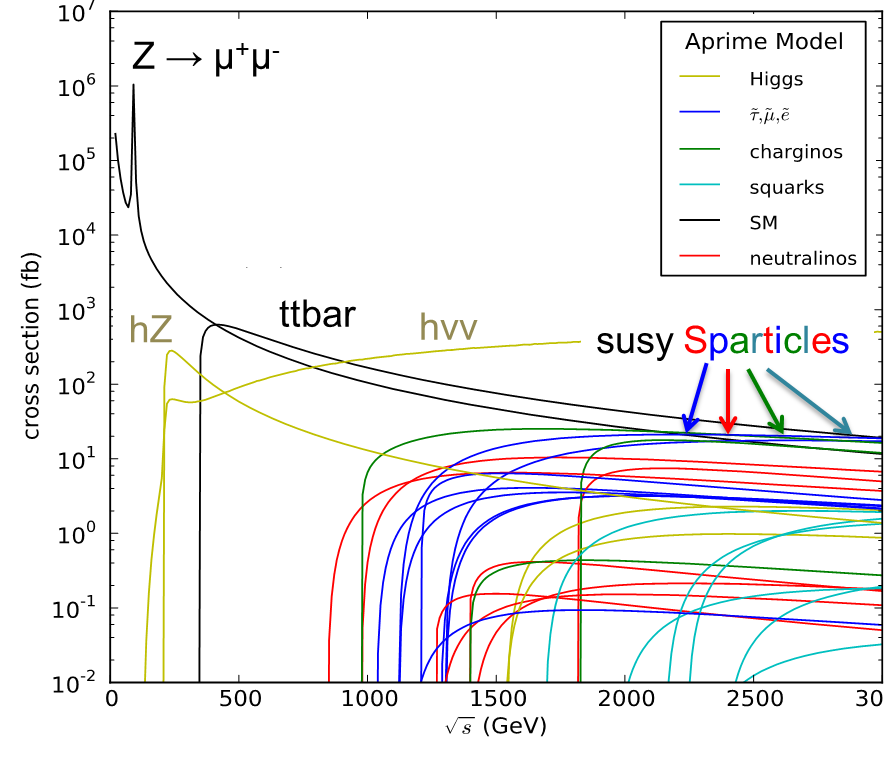
\includegraphics[width=6cm]{models}
\end{columns}
\end{frame}

\begin{frame}
\frametitle{Higgs measurements}
\centering
\begin{columns}[c]
\column{6cm}
\centering
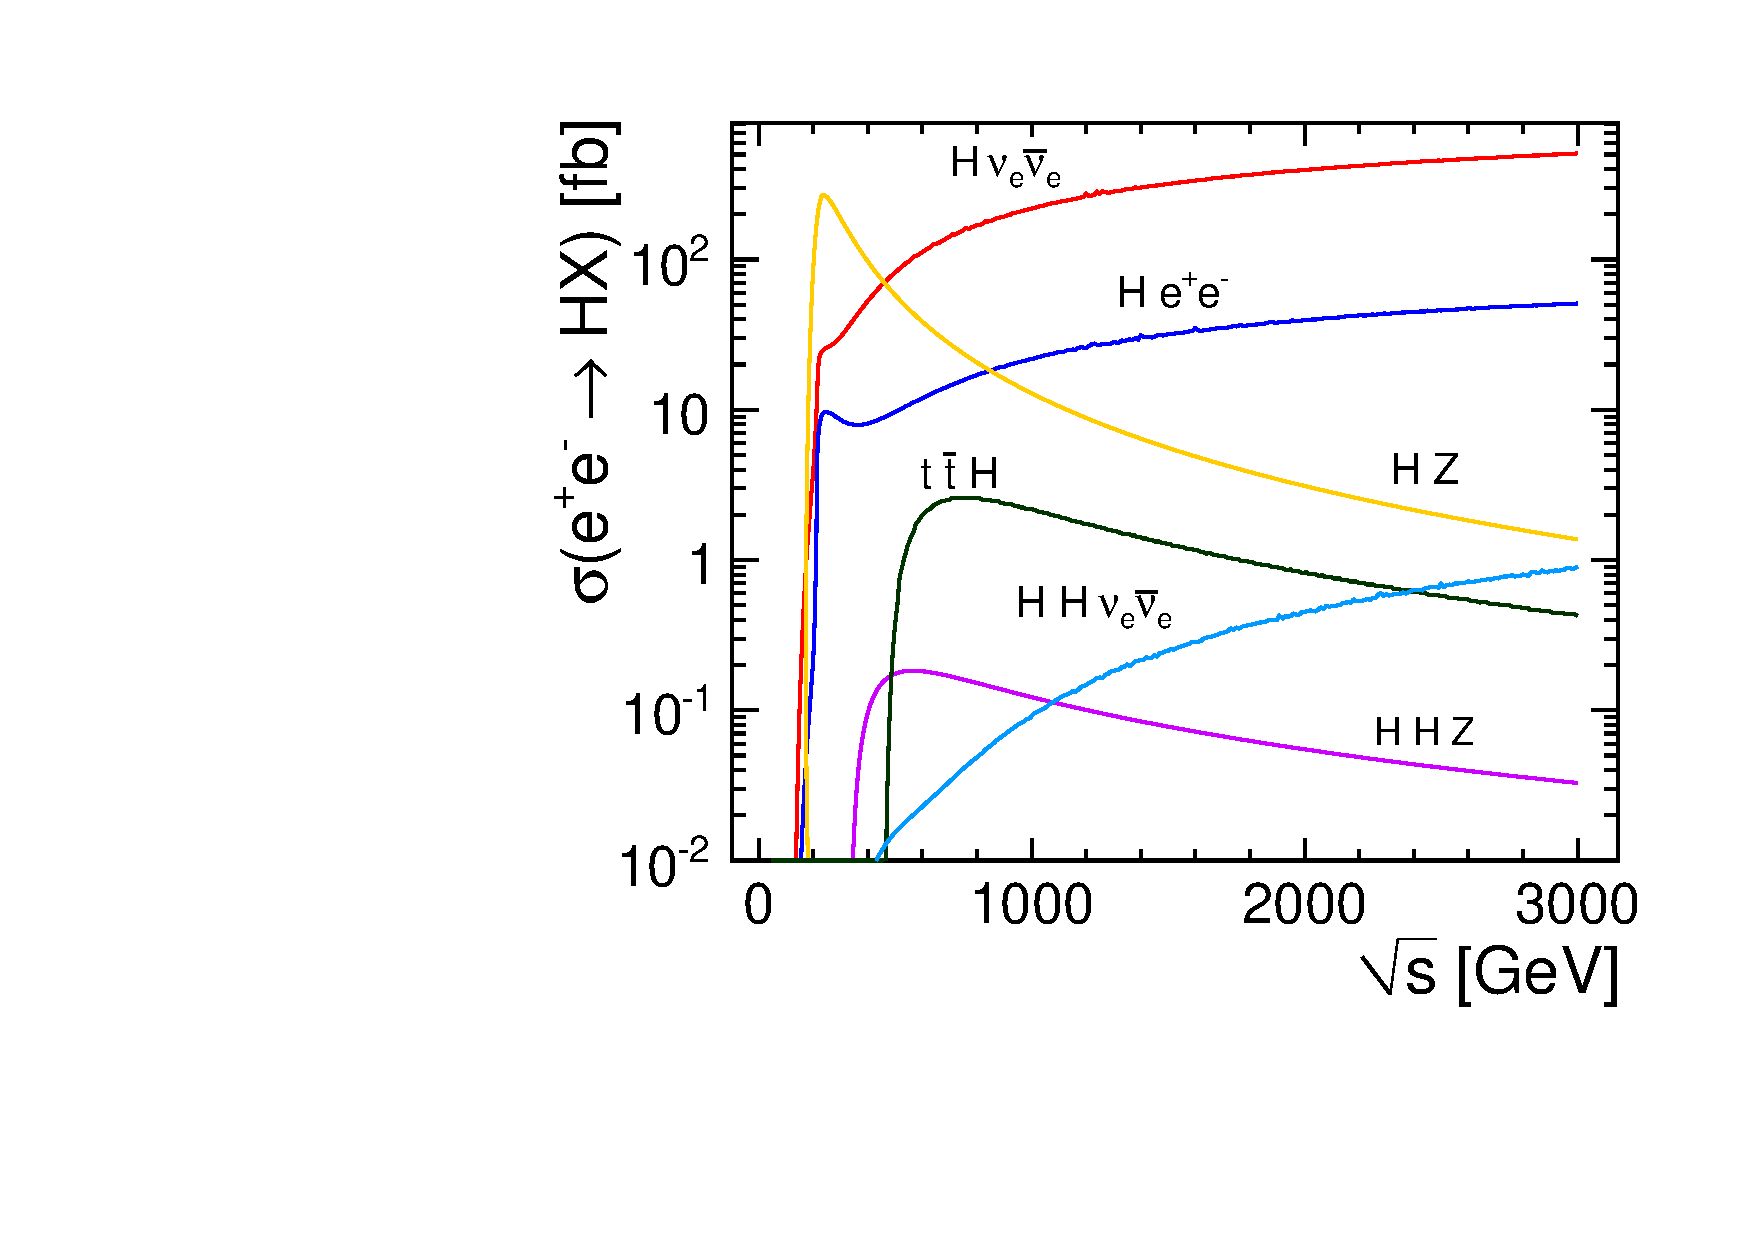
\includegraphics[width=4cm]{xsec_vs_cme}
\column{6cm}
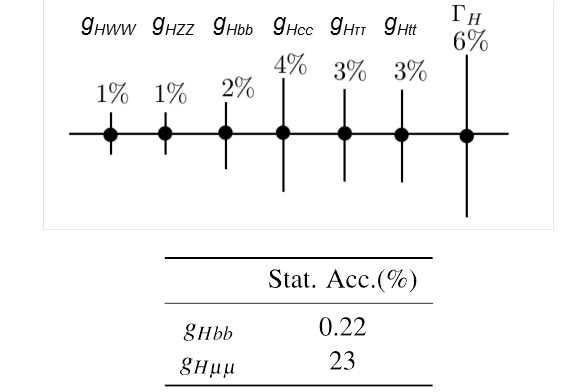
\includegraphics[width=3cm]{higgs}
\end{columns}
\begin{columns}[c]
\column{6cm}
\centering
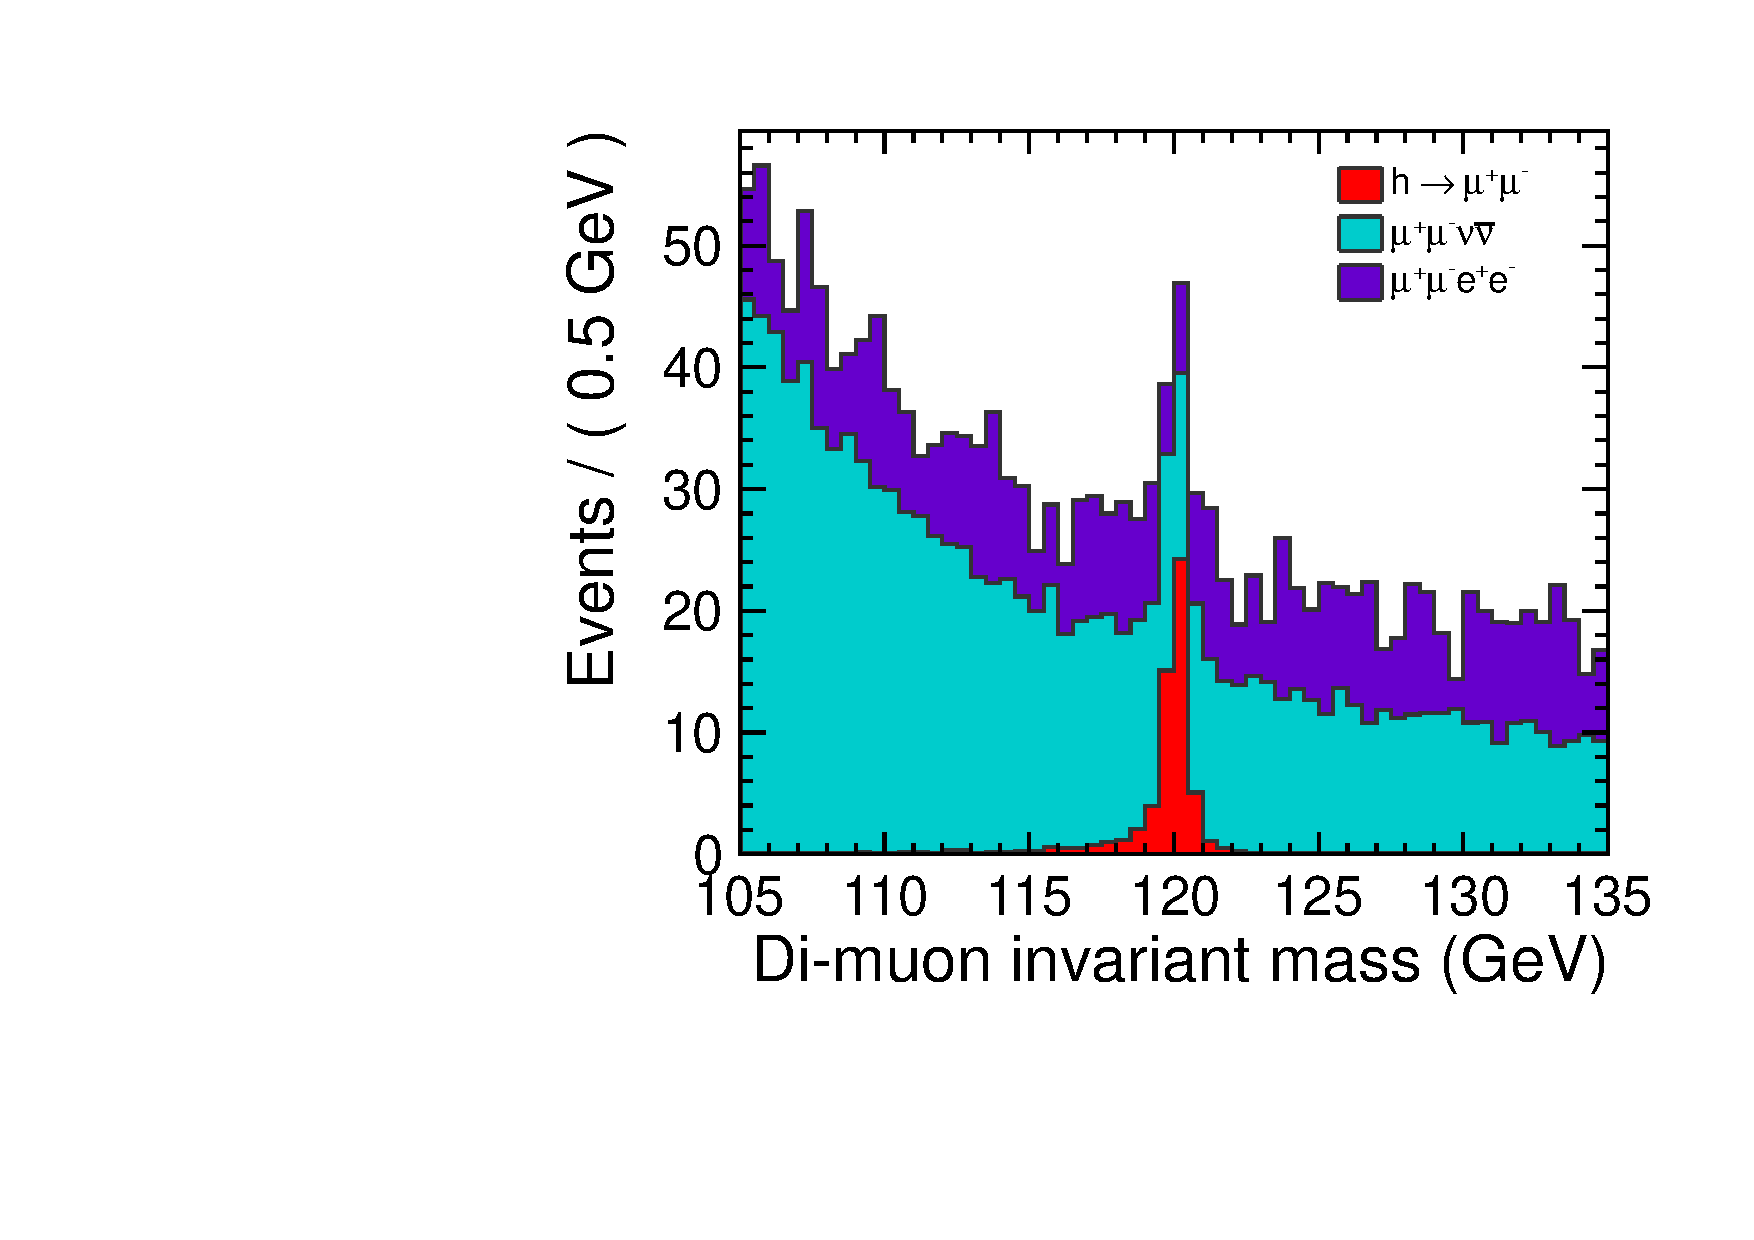
\includegraphics[width=5cm]{ee_h_mumu_mass_mh120GeV}
\column{6cm}
\centering
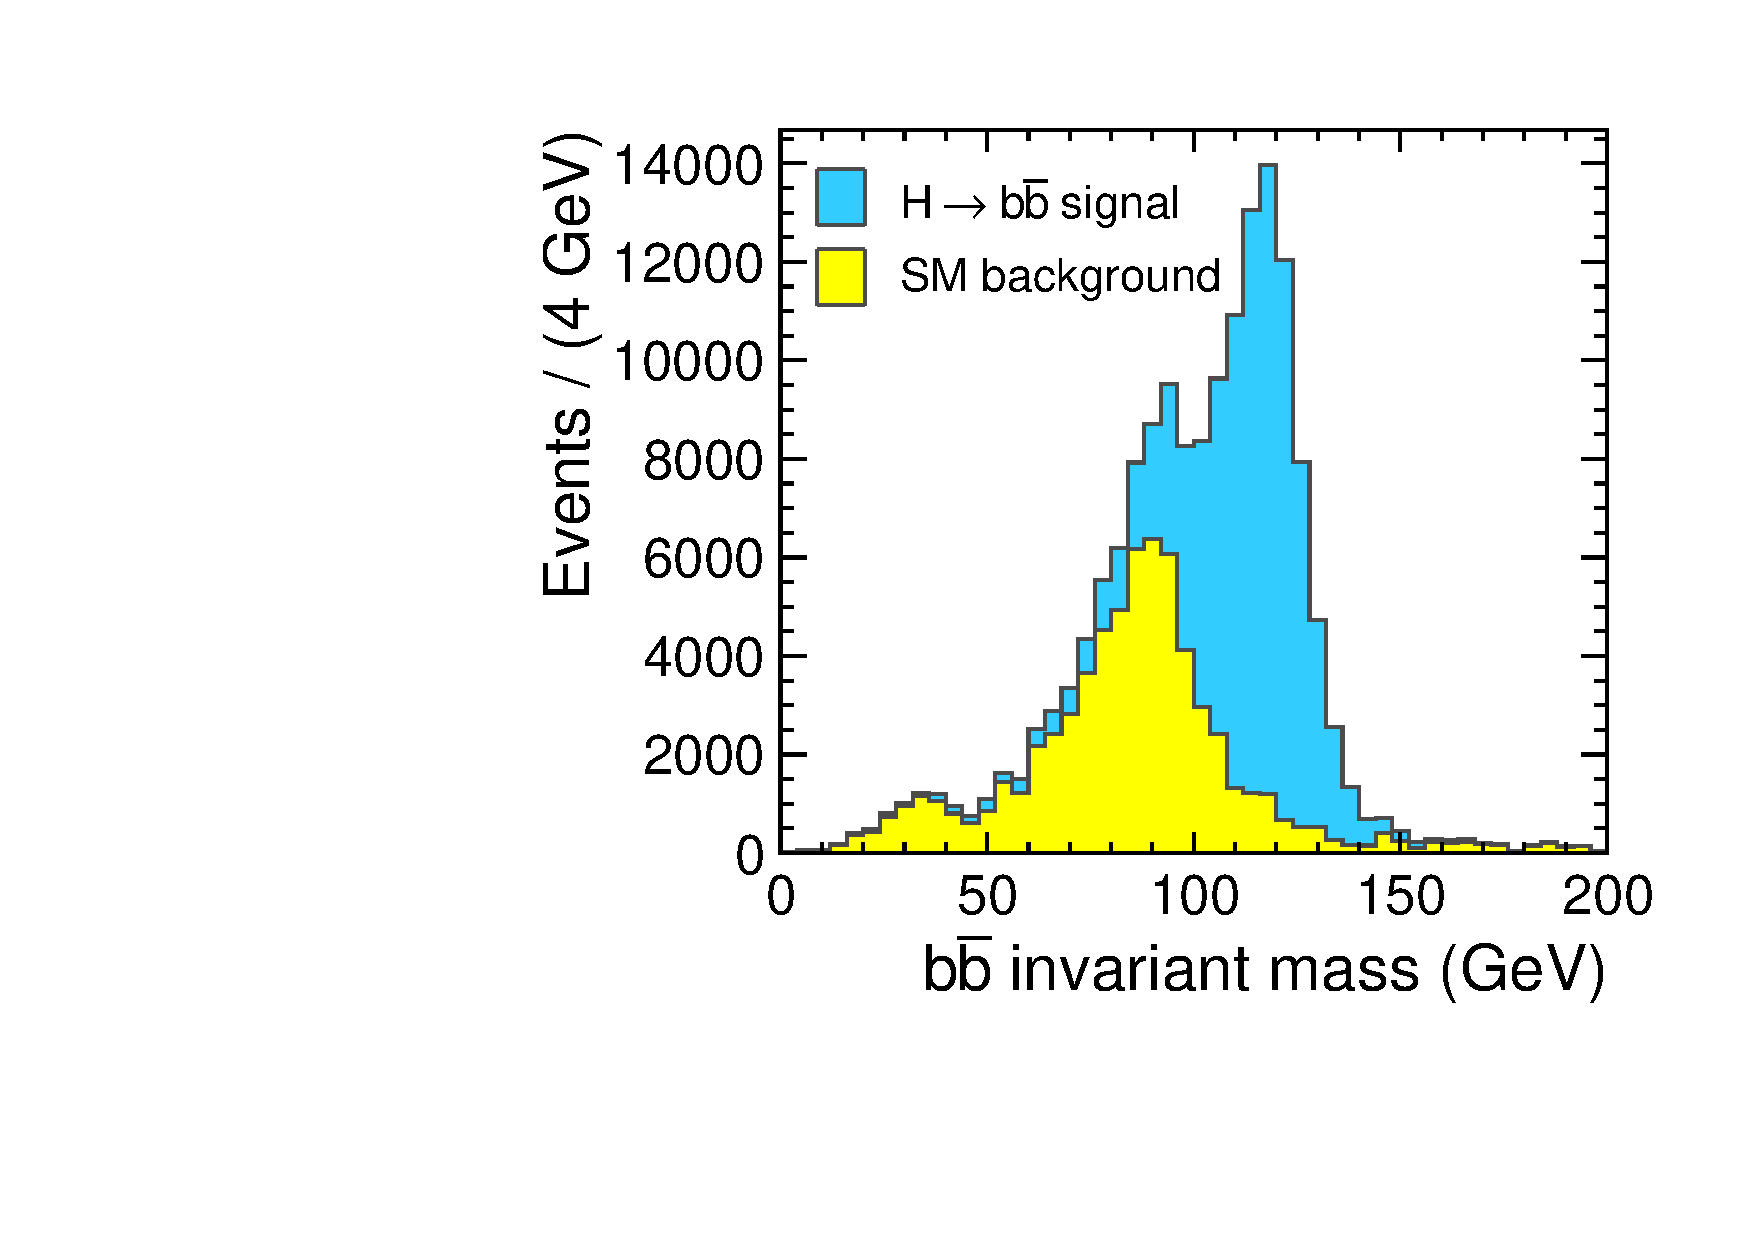
\includegraphics[width=5cm]{ee_h_bb_mass_mh120GeV}
\end{columns}
\end{frame}

\begin{frame}
\frametitle{Super Symmetry}
2 models considered to test several aspects: b-tagging, PFA, etc.
\begin{columns}[c]
\column{6cm}
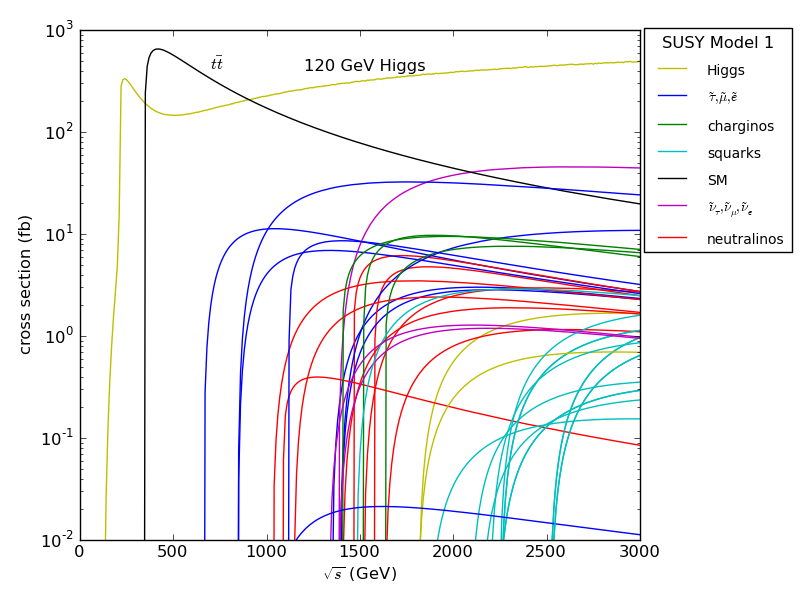
\includegraphics[width=6cm]{susy_model1}
\column{6cm}
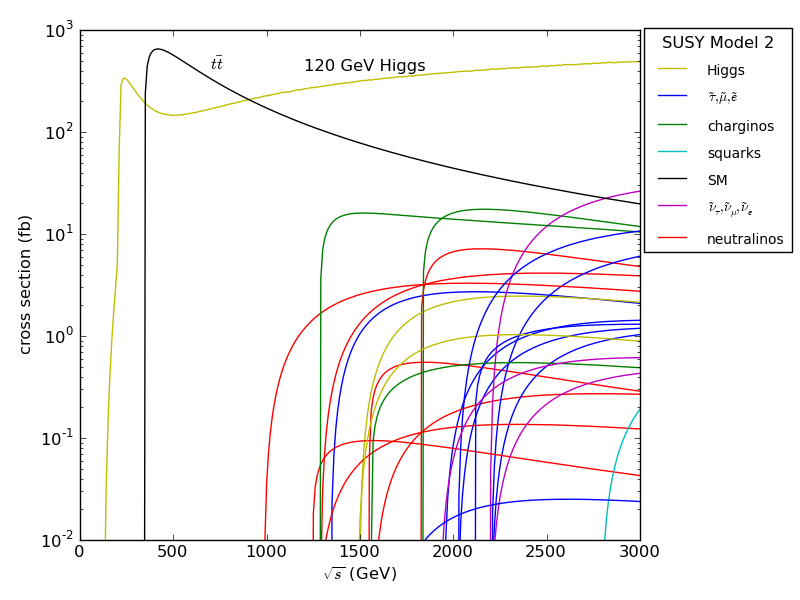
\includegraphics[width=6cm]{susy_model2}
\end{columns}
Test of Neutralino Dark Matter Hypothesis
\end{frame}

\begin{frame}
\frametitle{New physics scenarii}
\begin{itemize}
  \item Higgs strong interactions
  \item Z'
  \item Contact interactions
  \item Extra dimensions
\end{itemize}
\end{frame}

\section[CLIC]{A few words on the CLIC machine and beam} 
\begin{frame}
\frametitle{The CLIC accelerator}
general description, dimension, techno
\end{frame}

\begin{frame}
\frametitle{Technology choice}
\end{frame}

\begin{frame}
\frametitle{A particular beam structure}

\end{frame}

\begin{frame}
\frametitle{Running conditions}
overlay, pairs
\end{frame}

\section{The detectors}
\begin{frame}
\frametitle{The detector requirements}

\end{frame}
\begin{frame}
\frametitle{The CLIC\_ILD detector}
\end{frame}
\begin{frame}
\frametitle{The CLIC\_SID detector}
\end{frame}

\section[Bkg suppression \& phys. analysis]{Background suppression and physics
analysis}
\begin{frame}
\frametitle{Background suppression}
PFA timing cuts
\end{frame}

\begin{frame}
\frametitle{Use of PFA for physics analysis}
\end{frame}

\section[LCD for the DBD]{CERN LCD group in SiD DBD}
\begin{frame}
\frametitle{LCD group involvement in the SiD DBD}
ttH, production
\end{frame}

\section{Conclusions}
\begin{frame}
\frametitle{Conclusions}

\end{frame}
\end{document}